\documentclass[10pt, letterpaper]{article}  % Also try report, book, poem, slides, letter
\usepackage{geometry}
\usepackage{graphicx}
\usepackage{amsmath}
\usepackage{amssymb}
\usepackage{minted}
\usepackage{lipsum}
\usepackage{hyperref}
\usepackage{caption}
\usepackage{natbib}
% \usepackage{times}
\geometry{left=0.5in, right=0.5in, top=1in, bottom=1in}




\title{Super Cool Title}
\author{Daniel Szelogowski}
\date{\today}




% Everything above is the 'preamble'
\begin{document}

\maketitle

\tableofcontents
\clearpage  % Page break


\section{Introduction}

Here's some text

\subsection{Second Intro}

More Text

\subsubsection{Third Intro}

More text

\paragraph{Something else:} more stuff




% Get rid of numbering using *
\section*{No Numbers Here}

\section{Text Formatting}

Bold text: \textbf{Bold} \\  % Line break using \\
Italic text: \textit{Italic} \\
Underline text: \underline{Underline} \\
Monospace text: \texttt{TrueType} \\
\quad\quad      \verb|cool('wow')|

\begin{minted}{java}
class Hello {
    void main() {
        ...println("Hello, world!");
    }
}
\end{minted}

\noindent Footnote\footnote{Cool beans}

\begin{center}
    This text is centered
\end{center}



\section{Lists}

\begin{itemize}  % Bulleted List
    \item Thing
    \item Thing
    \item Thing
    \begin{itemize}
        \item Nested
    \end{itemize}
\end{itemize}

\noindent \hrulefill{}

\begin{enumerate}  % Numbered List
    \item Thing 1
    \item Thing 2
\end{enumerate}


\section{Images}

\begin{figure}[h]  % here
    \centering
    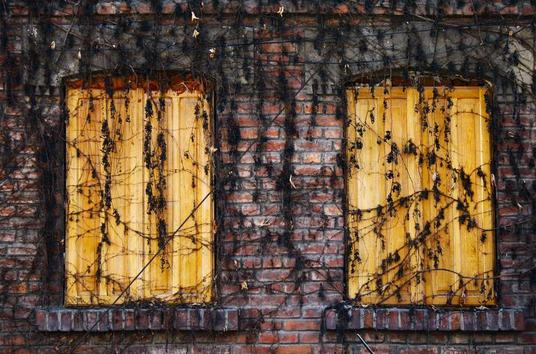
\includegraphics[width=0.75\linewidth]{images/image.jpg}
    % usepackage caption
    % \captionsetup{labelformat=empty}
    % \caption*{A thing}
    \caption{A thing}
    \label{fig:house1}
\end{figure}


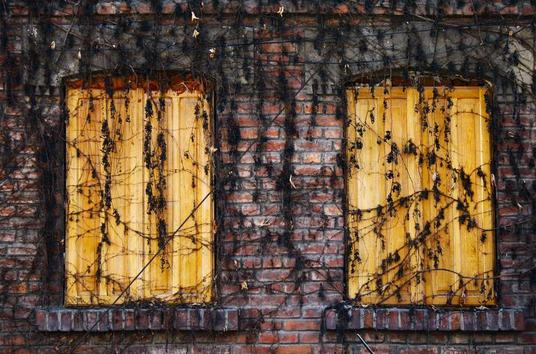
\includegraphics[width=2in]{images/image.jpg}

Also see \textbf{Figure \ref{fig:house1}} or the
\hyperref[sec:math]{Math Section}.

You might want to click \href{http://test.com}{this link} or visit \url{http://test.com}.



\section{Math}
\label{sec:math}

Inline math using \$ symbols: $\pi = 3.14159$

Block math:

\[
    \sum^{5}_{i=1} i^2
\]

% Also see \begin{equation} or \begin{equation*}
\begin{align*}
    x &= 5 \\
    y &= 7 * 1 / 2 \\
    z &= 3 + 5
\end{align*}


\vspace{3in}
\section{Tables}

\begin{table}[h!]
\centering
\begin{tabular}{|c|c|c|}
    \hline
    c1 & c2 & c3 \\
    \hline
    c4 & c5 & c6 \\
    c7 & c8 & c9 \\
    \hline
\end{tabular}

\vspace{-0.3cm}
\caption{Cool table}
\end{table}

\begin{small}
    really small text
\end{small}



% Place text from file exactly here
\section{Cool Beans}
These are some cool beans.

% Place text from file starting on its own page; good for chapters
\section{Cool Beans}
These are some cool beans.



\section{Lorem Ipsum}
\lipsum[1-5]
According to \cite{Goodfellow_Goodfellow_Wilson_Hunt_2010}, here's some additional text. Also something else \citep{Szelogowski_2022}. Also ``quotes'' here. (or use csquotes package)

% \cite is for when the author name is part of the text
% \citep puts the entire citation in ()s



% bibcitation.com

\pagebreak
\bibliographystyle{apalike}  % Also see plain and plainnat
\bibliography{references}



\end{document}
